%
%
%
\begin{document} \maketitle


\section{Introduction} 
\label{introduction}
       
A RPG (Role Playing Game) is game where player assumes the role of on the character. A RPG is usually story driven and the character usually has quest to complete. In the course of the game the player will go to different environments such as town and dungeons. In they these environments the player will have to battle opponents in battles. Combat in RPGs is normally a simple turn based system where player and the opponents take turns attacks each other using various skills. 

A Tactical RPG is sub-genre of an RPG that focuses on the combat side of the genre. A Tactical RPG is series of \texttt{battles}, which take place in various environments intertwined with an over-aching story.

Each \texttt{battle} is grid based (like chess) where each player has a number of units(pieces). 
\begin{figure}
	[htbp] \centering 
	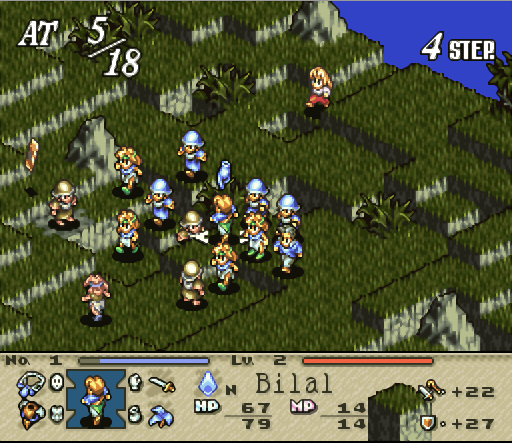
\includegraphics[height=3in]{figures/TRPG.png} \caption{\textbf{Tactics Ogre}\cite{to} a classic Tactical RPG } \label{fig:figures_TRPG} 
\end{figure}
The players taken turns to moves their units. Each unit has attributes associated with it such as strength, and hit points that affect all the actions in the game. Like chess there are different kinds of units which affects how the unit moves and what action they can perform. A unit can attack other player's units, the goal of the battle is usually to defeat all the opponents units.

The aim of this project is to create a engine which will take resources such as graphics, sound and rules of the game to create a runnable Tactical RPG.

\section{Objectives}
\subsection{Primary}
\label{primary}
The main goal of the primary objectives is allow the user to create a complex Tactical RPG, with limited customisability.  
\begin{itemize}
\item To develop an engine that takes:
\begin{itemize}

 \item The definition of character attributes and a combat system.
	\item The definition of a world broken up into the smaller environments.
	\begin{itemize}
		\item The rules of the game.
		\item The kinds of enemies.
	\end{itemize}
	
	\item The definition of simple story as a wrapper for the whole game, from the start to the conclusion of the game
	\begin{itemize}
		\item Which is told between the movement between different environments.
	\end{itemize}
	                        
	\item The set of selected character attributes.
	
\end{itemize}
and create a playable tactic RPG.

\item To include in the engine support for the following:
\begin{itemize}
	\item \texttt{units} with a fixed set of associated attributes such as:
	\begin{itemize}
		\item Hit-points (which represent the health of the unit).
		\item Strength.
		\item Defence.
		\item Move (The number of tiles the unit can move each turn).
	\end{itemize}
	
	\item \texttt{battles} which take place on grid and include:
	\begin{itemize}
		\item A set number of \texttt{units} for each player.
		\item A Winning \texttt{condition} such as defeat all of the other players units.
		\item Battles are \texttt{turn based} meaning that each player moves all their units (once) before the next player turn.   
		\item A combat system.
	\end{itemize}
	
	\item A combat system that includes
		\begin{itemize}
			\item \texttt{combat} between adjacent units.
			\begin{itemize}
				\item When the unit hit-points are reduced to zero they are \texttt{defeated} and are removed from the map
			\item A set of rules that govern the combat.
			\end{itemize}
			
		\end{itemize}
	
	\item A predefined set of behaviours for how the non-player characters should behave.
	\begin{itemize}
		\item Including pathfinding.
	\end{itemize}
	
	\item A simple graphical representation of of the game.
	\begin{itemize}
		\item Which is show the grid with all the units.
		\item Allow the user to move their units and see the opponents moves.
		\item Allows the user to attack the opponents units.
		\item Text will be to describe the more complex actions such magic.
	\end{itemize}
\end{itemize}
\end{itemize}

\subsection{Secondary}
\label{secondary}
The main goal of the secondary objectives is allow the user more customisability. 
\begin{itemize}
	\item Tile \texttt{height}, where units can only move to tiles of a smilier height.
	
	\item Tiles that are not passable such as sea, lava, etc.
	
	\item Tiles have different movement costs associated with them.
	
	\item Isometric graphics view of the game.
	
	\item Long distance weapons\slash magic for player and AI.
	
	\item Direction and height of the character's tile affects attack.
	
	\item Sound effects.
	
	\item Music.
	
	\item Saving and loading games.
	
	\item Allow the user to specify some of behaviour of non-player characters
	\begin{itemize}
		\item Through the use of scripting.
		\item An example: always attack a certain kind of unit or always attack the unit with the least Hit Points.
	\end{itemize}
	
	\item A graphical view to allow user specify the input to the engine.
\end{itemize}

\subsection{Tertiary} 
\label{tertiary}
The goal of the Tertiary objectives are provide the user with more customisability and to provide a GUI for simple scripts. 

\begin{itemize}
	\item Custom events
	\begin{itemize}
		\item Attached to units or titles, could be used for:
		\begin{itemize}
			\item Making the player win if some enemies unit has less then 50\% Hit Points.
			
			\item Damaging a character if step on a specified.
			
			\item Showing some part of the story when a player's character reach a specified tile.
		\end{itemize}
	\end{itemize}
	
	\item A graphical editor for making custom maps, events and specifying the input to the engine.
	\begin{itemize}
		\item The gui would also be able to create the scripts for simple event such as `Defeat the leader' as a winning condition.
	\end{itemize}
	\item Animations for units and movement.
\end{itemize}

\subsection{Ethical Considerations} 
\label{ethicalconsiderations}
\begin{itemize}
	%\item Form by 28th October.
	
	\item Collection of data from questionnaire.
	\begin{itemize}
		\item Just result of questionnaire, no personal data.
	\end{itemize}
	
	\item Asking users to create a game.
	
	\item Asking users to play the created game.
\end{itemize}

\subsection{Questionnaire}
\begin{enumerate}
	\item Have you played a Tactical RPG before?
	\begin{enumerate}
		\item If yes, did Engine have features you like to create in a game?
	\end{enumerate}
	\item How easy to use was the Engine?
	\item What particular aspects of the Engine did you like? 
	\item What particular aspects of the Engine did you dislike? 
	\item Any comments?
\end{enumerate}

\clearpage
\subsection{Survey}
%CS4099 Dissetation
%!TEX root = ../Project.tex
\section{Questionnaire}
\label{sec:questionnaire}
\subsection*{Task}

The task involves creating a single level of a Tactical RPG (Each level is grid based (like chess) where each player takes turns to move and/or attack the opposing player).   

\subsubsection*{Weapons}
\begin{center}
\begin{tabular}{c|c|c|c|}
	Name        & Weapon Type & Strength & Icon \\\hline
	Long Bow    & Ranged      & 30       & 
\includegraphics[height=0.5cm]{figures/bow.png}   \\ 
	Black Spear & Spear       & 20       & 
\includegraphics[height=0.5cm]{figures/spear.png} \\ 
	Ice Sword   & Melee       & 10       & 
\includegraphics[height=0.5cm]{figures/sword.png} \\ 
\end{tabular}
\end{center}

\subsubsection*{Skills}
\begin{center}
	\begin{tabular}{c|c|c|c|c}
		
		Name          & Type   & Range & Area & Strength \\\hline
		Air Blade     & Ranged & 2     & 0    & 25       \\ 
		Thunder Flare & Ranged & 4     & 1    & 15       \\ 
	\end{tabular}
\end{center}


% Makes a unit
\newcommand{\unit}[7]{\begin{tabular}{|p{1cm}|lp{2cm}|}
\hline
\multicolumn{3}{|c|}{#1} \\
\hline
\multirow{6}{*}{\includegraphics[height=1.7cm]{figures/#2}} 
 & Weapon    & #3 \\
 & Strength  & #4 \\
 & Move      & #5 \\
 \cline{2-3}
 & \multicolumn{2}{c|}{Skills} \\
 \cline{2-3}
 \ifstrempty{#6}{}{\foreach{\unitSkill}{}{#6}}
 & \multicolumn{2}{l|}{#7}\\
\hline
\end{tabular}
}

\newcommand\unitSkill[2]{
	& \multicolumn{2}{l|}{#2}\\
}
\subsubsection*{Units}
\unit{Agrias}{unit1.png}{Long Bow}{20}{3}{}{Air Blade}
\hspace{0.5cm}
\unit{Elena}{unit4.png}{Black Spear}{30}{5}{}{Thunder Flare}

\subsubsection*{Map Enemies}
\unit{Mustadio}{unit2.png}{Long Bow}{20}{3}{}{}
\hspace{0.5cm}
\unit{Druksmald}{unit3.png}{Ice Sword}{30}{5}{}{}
\\[0.5cm]
\unit{Zalbaag}{unit3.png}{Ice Sword}{25}{5}{}{}
\hspace{0.5cm}
\unit{Ajora}{unit3.png}{Ice Sword}{20}{5}{}{}


\clearpage
\subsubsection*{Map}
\begin{figure}[h!]
	\centering
		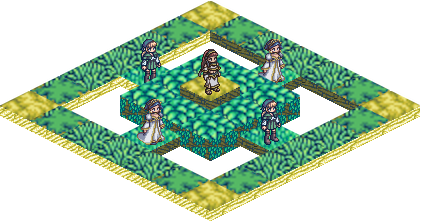
\includegraphics[height=2.7in]{figures/Task.pdf}
	\caption{The map to create}
	\label{fig:figures_Task}
\end{figure}


\paragraph{Win Condition\\}
Defeat Specific Unit   -- Elena.

\paragraph{Start Dialog:}
\begin{itemize}[topsep=0mm,noitemsep]
	\item[Text]  You can not Win!
	\item[Speaker] Kyou
\end{itemize}

\paragraph{End Dialog:}
\begin{itemize}[topsep=0mm,noitemsep]
	\item[Text]  How did I lose?
	\item[Speaker] Elena
\end{itemize}

\paragraph{Music:\\}
Background Music 3-15 Faraway Heights

\clearpage
\subsection{Editor Usability Scale}
{\footnotesize © Digital Equipment Corporation, 1986.}\\

\startingQuestion{I think that I would like to use this system frequently.}

\question{I found the system unnecessarily complex.}

\question{I thought the system was easy to use.}

\question{I think that I would need the support of a technical person to be able to use this system.}

\question{I found the various functions in this system were well integrated.}

\question{ I thought there was too much inconsistency in this system}

\question{I would imagine that most people would learn to use this system very quickly}

\question{ I found the system very cumbersome to use}

\question{ I felt very confident using the system}

\question{  I needed to learn a lot of things before I could get going with this system}

\subsection{Playing a pre-created game}

\startingQuestion{I found the game intuitive}

\question{The game had a appropriate level of difficulty. }

\question{I enjoyed playing the game.}

\fquestion{Please share any comments about the game :}


\clearpage
\subsection{Questions}
\fquestion{Have you played a Tactical RPG before?}

\fquestion{Did Engine have features you like to create in a game?}

\fquestion{How easy to use was the Engine?}

\fquestion{What particular aspects of the Engine did you like?}

\fquestion{What particular aspect of the Engine did you dislike?}

\fquestion{What features would you like to see added to the Engine in the future?}

\fquestion{Please share any other comments:}



\clearpage

\subsection{Resources} 
\label{resources}
\begin{itemize}
	\item None.
\end{itemize}



\bibliography{Citations}
\end{document}
